% DESCRIBE BRIEFLY THE HAND

There are several ways to implement underactuation in a humanoid hand. We are particularly intereseted in the adaptive synergy transmission due to its simplicity and robust design, yet complex interaction with the environment. The Pisa/IIT SoftHand~\cite{Catalano2014Adaptive} exhibits one of such transmissions.

The hand has 19 degrees of freedom distributed in
four fingers and an opposable thumb, and only 1 degree of actuation. The synergy motion derives from human postural databases. The overall behavior parameters are the matrices that correspond to the transmission ratio,~$R$, to the joint stiffness,~$K_q$. The actuation is done through a single tendon routed throuhout all joints, making the fingers to flect and abduct.

% THE LACK OF SENSORS AND FUTURE LARGE DATASETS REQUIRED JUSTIFY THE USE OF SIMULATED DATA

Moving such a hand to grasp an object results in a hard-to-predeict contact and hand shapes due to the adaptivity. To the purpose of this work, we are intereseted in generating examples of this kind. However, recording the trajectory of all bodies into play in a real scenario is not a banal thing when dealing with cluttered and small spaces where human-sized grasps take place, specially if hundreds are required. For this reason, we have opted to generate the examples using a rigid-body dynamic simulator, where these problems are overcome, however, others arise. The main two elements are the contact stability and the hand behavior, which in this case, the latter depends heavily on the former. We are using the standard distribution of Gazebo and Open Dynamic Engine, both widely spread with recognized performance.
% but not perfect. There is an on-going work on improving the mesh-to-mesh collision there.
Regarding the second element, the adaptive synergy equations have been implemented as a plugin which accompanies the proper kinematic description of the Pisa/IIT SoftHand\footnote{The Pisa/IIT SoftHand ROS/Gazebo packages are available at \url{https://github.com/CentroEPiaggio/pisa-iit-soft-hand}}.

\begin{figure}
  \centering
  \begin{tabular}{ccc}

  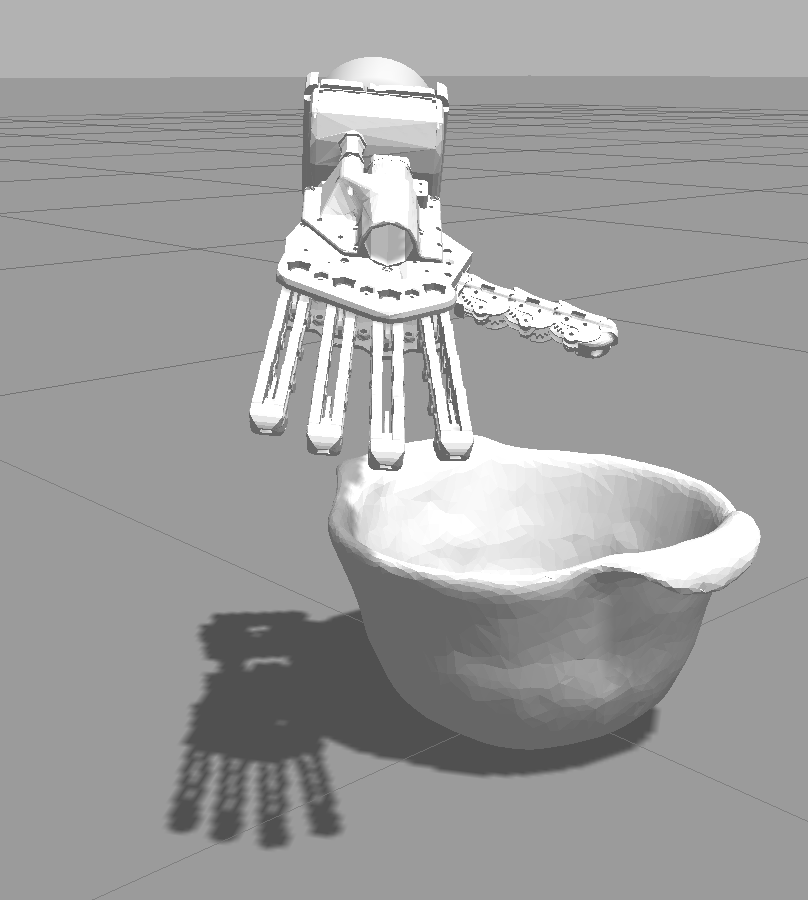
\includegraphics[width=0.3\linewidth]{containerB_pinch_1.png} &

  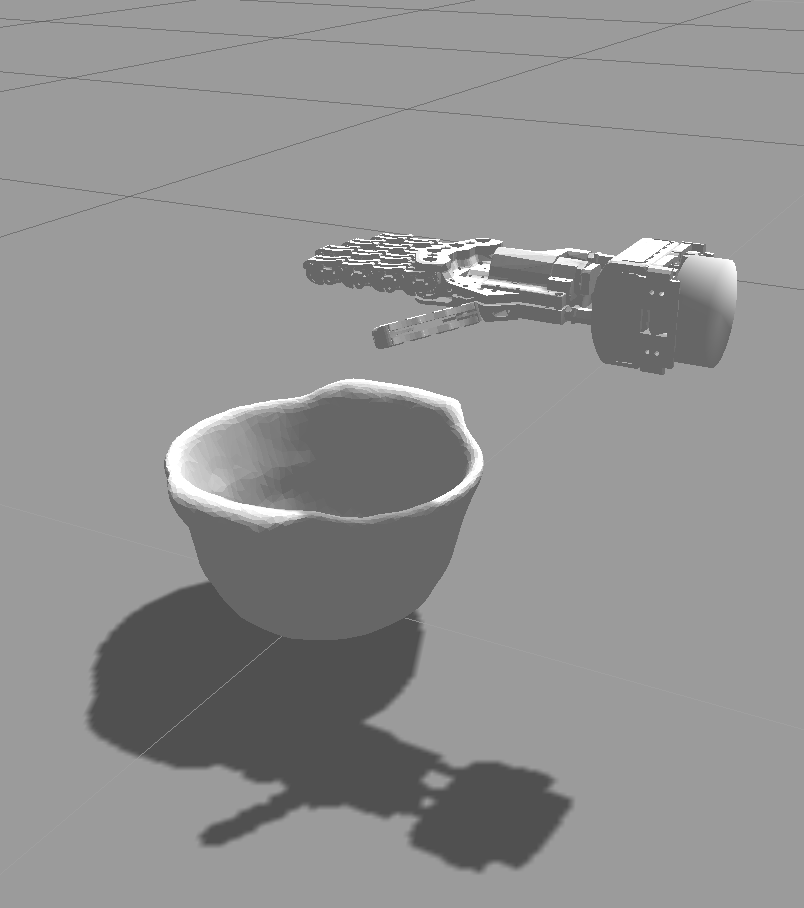
\includegraphics[width=0.3\linewidth]{containerB_rim_1.png} &

  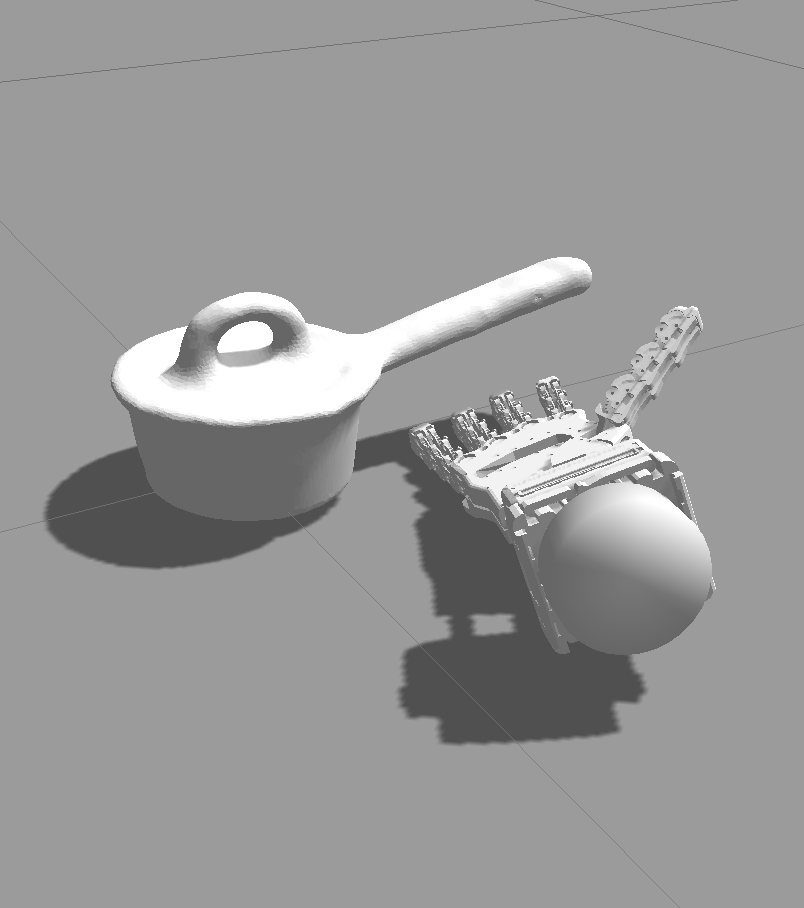
\includegraphics[width=0.3\linewidth]{pot_1.png} \\

  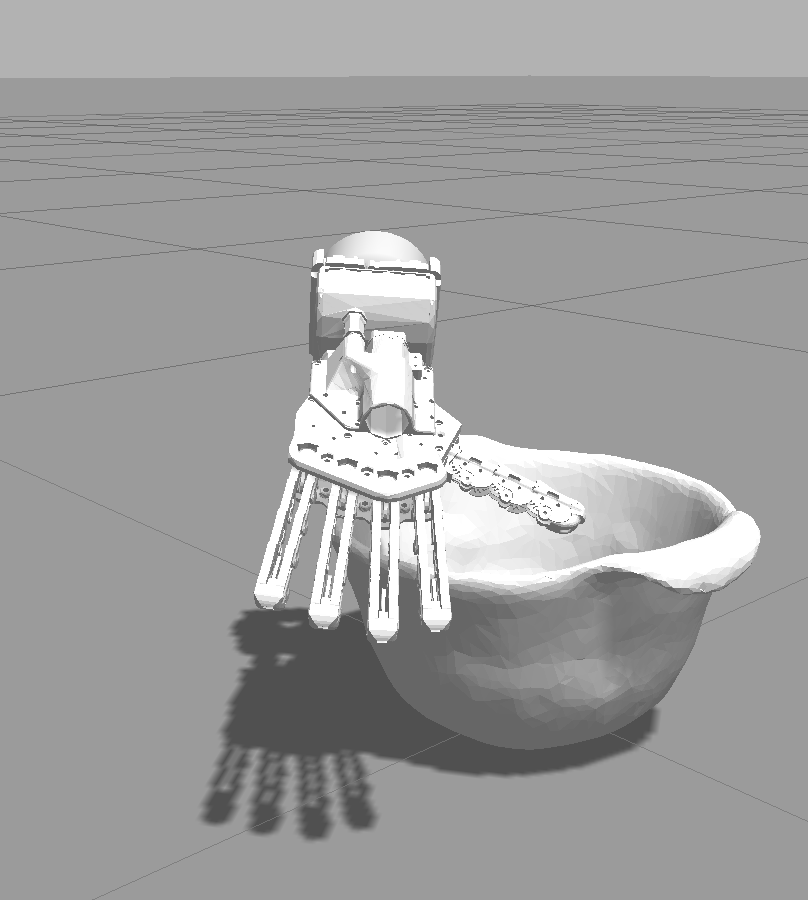
\includegraphics[width=0.3\linewidth]{containerB_pinch_2.png} &

  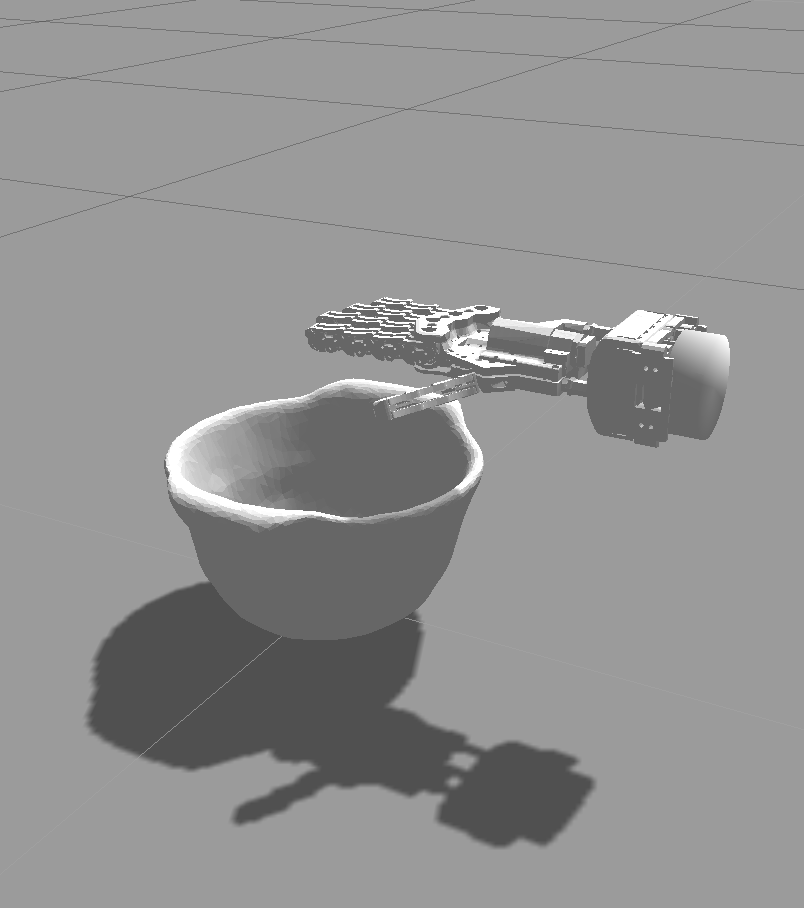
\includegraphics[width=0.3\linewidth]{containerB_rim_2.png} &

  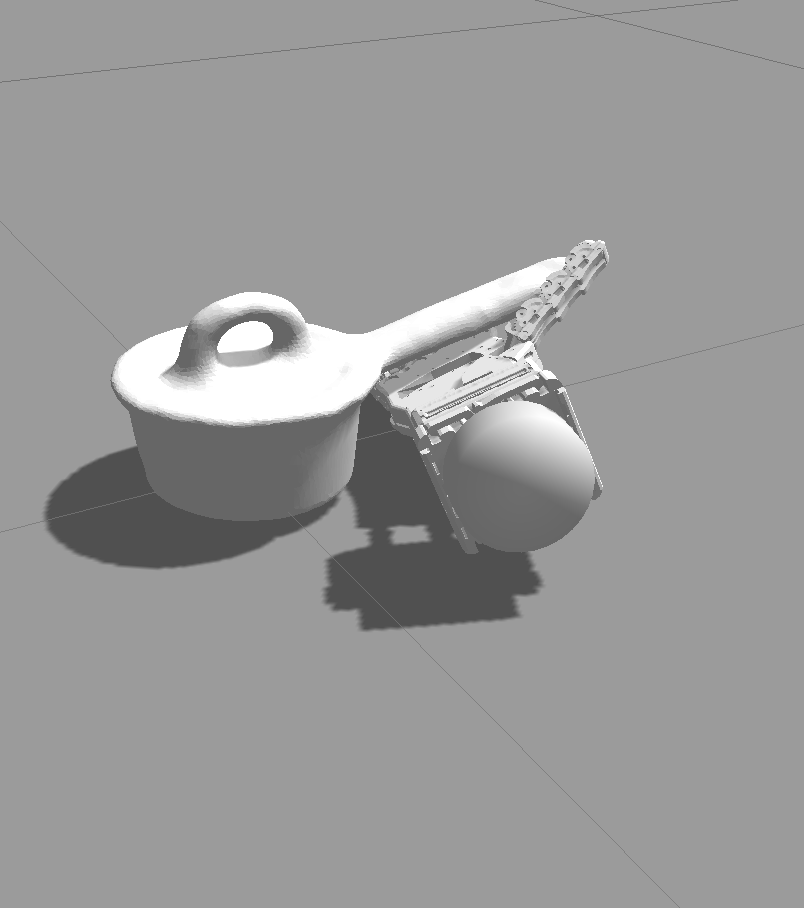
\includegraphics[width=0.3\linewidth]{pot_2.png} \\

  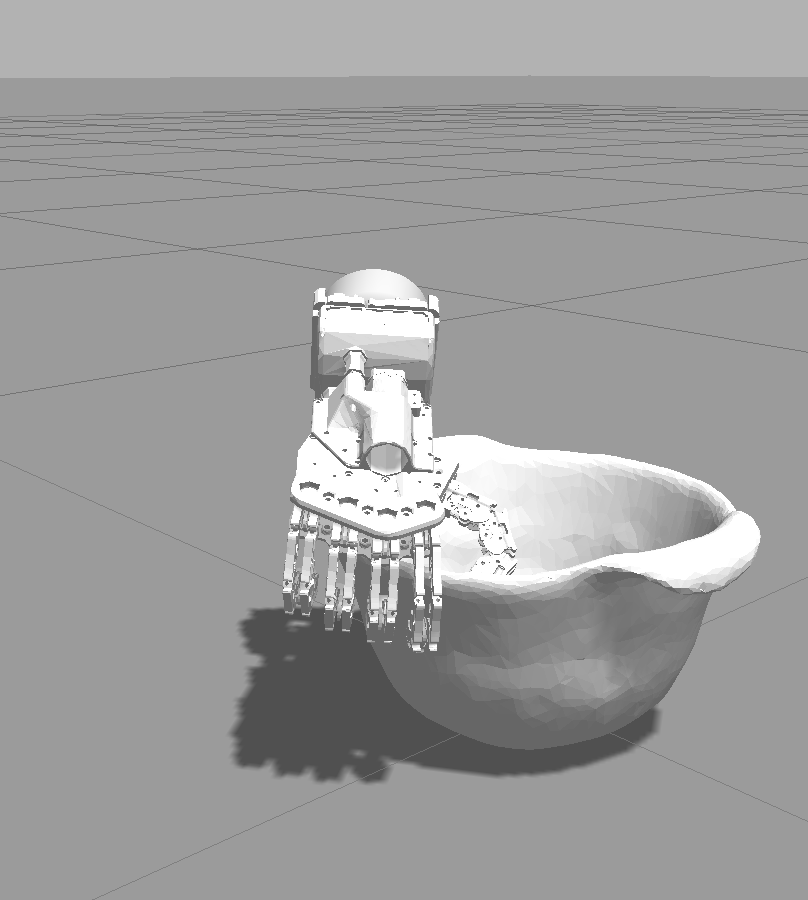
\includegraphics[width=0.3\linewidth]{containerB_pinch_4.png} &

  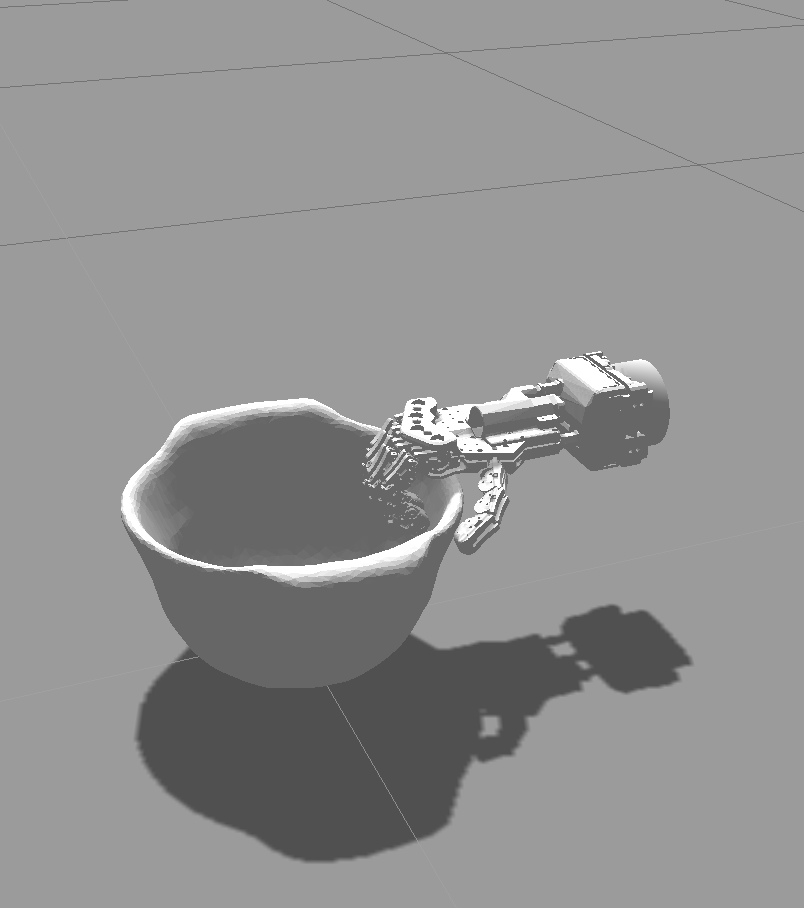
\includegraphics[width=0.3\linewidth]{containerB_rim_4.png} &

  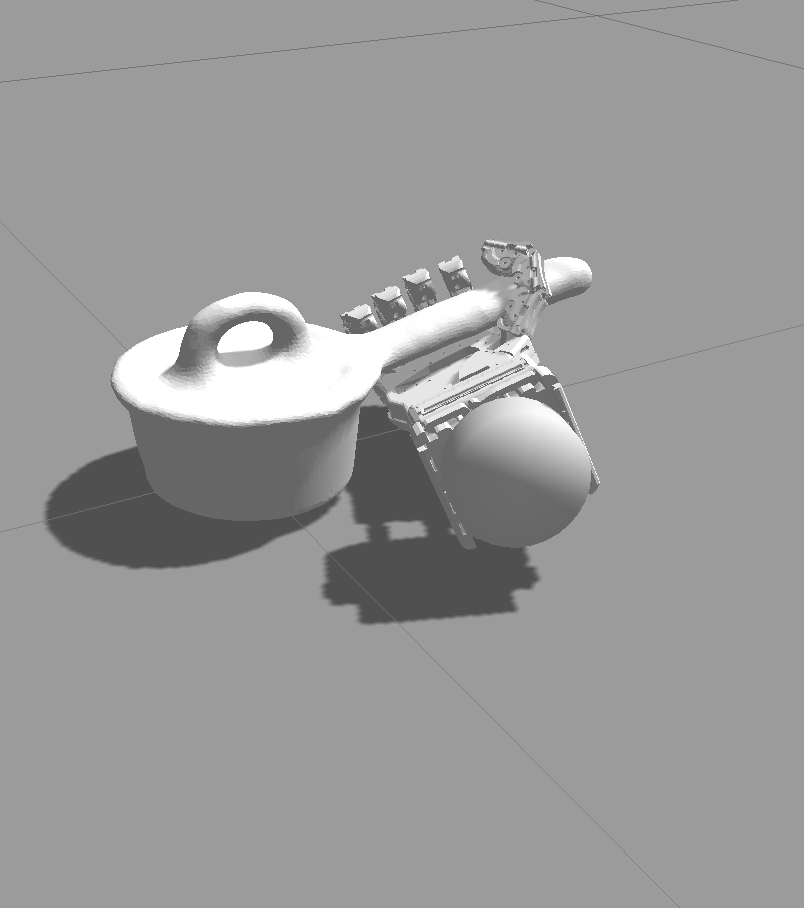
\includegraphics[width=0.3\linewidth]{pot_3.png} \\

  \end{tabular}

  \caption{Snapshots of the simulation of a pinch and rim grasp types for the colander (first and second columns), and handle grasp for the pot (last column).}
  \label{fig:simulations}
\end{figure}

% HOW WE GENERATED THE DATA

At the current state, there are no generally accepted measures concerning whether an object being grasped by an underactuated adaptive hand  is good or not, hence the lack of robust grasp planners for them is not a surprise. Thus, generating a large dataset at this point is useless, and there are plans in the future to cover this area. As a result, we generated the examples by guiding manually the hand to a ``nice'' grasp as shown in Fig.~\ref{fig:simulations}. In this simpler scenario, we assume without lost of generality that the grasps are labeled by type. In our example dataset, we have three grasp types namely pinch, rim and by-the-handle. The main difference between pinch and rim is the fingers configuration w.r.t. the top border of objects. In the pinch grasp, the thumb goes inside whereas in teh rim grasp, the fingers go inside. In the latter, the container can be filled with liquid while holding, for instance.

For each grasp example, the corresponding dataset comprises the set of body trajectories, expicitly their position,~$p_i(t) \in \mathbb{R}^3$, and orientation,~$q_i(t) \in SO(3)$, over time for $i=1,\ldots,m$ bodies (including hand links), and the associated set of hand configurations,~$h_c(t) \in R^{n}$, with $n$ the hand degrees of freedom.

% FOR FUTURE WORK?

% Another challenge is to learn how any adaptive synergy transmission behave for any given kinematic design. 

%% BECAUSE I'M WORKING IN GENERATING DATA FOR ANOTHER COMPLIANT HAND BESIDES THE PISA SOFTHAND